\section{E-Meter}
The E-Meter, short for electricity meter, fulfills the role of monitoring all power consumed for a given customer. The PICA E-Meter exists as a replacement for the standard electricity meter, seen in figure \ref{fig:mechanical_meter}, found outside most homes and businesses. As the PICA E-Meter will replace an already existing piece of technology, the PICA E-Meter must fulfill all the same roles as a traditional power meter. In addition, team PICA seeks to provide extended capabilities, such as wireless meter reading and tamper detection.

Since the average consumer does not actually own the physical metering hardware, this portion of our senior design project targets the electric companies. We hope that by providing more accurate readings, more reliable meters, and more convenience the PICA E-Meter could entice some, if not all of the electric utility providers who still rely on traditional electric meters. The PICA E-Meter should cost less than \$200 each fully assembled. Team PICA currently cannot verify how this price compares to that of a traditional power meter, as they are not available on the open market.

The PICA E-Meter design functions for either 3-phase of 1-phase power, usually found in commercial or residential applications respectively. Both devices share the majority of the hardware, with only a different input board the main hardware functions identically for both applications.

\subsection{Original Ideas}
Early in the project team PICA decided to use a \ac{TI} MSP430 low-power microprocessor. The family of MSP430 devices includes several devices that could perform the necessary tasks, however, the MSP430F471xx family of devices are tailored for metrology. After some investigation the team decided to use an MSP430F47197 microprocessor as the core of the E-Meter. A summary of the specifications for this micrprocssor follows in table \ref{tab:msp430f47197_specs}.
{
\begin{longtable}[c]{|l|l|}
\caption{Specifications for the MSP430F47197\cite{slas626c}\label{tab:msp430f47197_specs}}\\
\hline
\rowcolor{lightgray}
Specification & MSP430F47197\\\hline
\endfirsthead
\caption[]{Continued from previous page}\\

\hline
\rowcolor{lightgray}
Specification & MSP430F47197\\\hline
\endhead
\multicolumn{2}{r}{{Continued on next page}}\\
\endfoot

\endlastfoot

Frequency                    & 16 MHz\\\hline
Flash                        & 120 kB\\\hline
RAM                          & 4 kB\\\hline
GPIO                         & 68\\\hline
Pin/Package                  & 100LQFP\\\hline
LCD Segments                 & 160\\\hline
ADC                          & 7 16-bit Sigma Delta\\\hline
Other Integrated Peripherals & Comparator, DMA, Hardware Multiply, SVS\\\hline
End Equipment Optimization   & Energy Meter\\\hline
Interfaces                   & 2 USCI\_A, 2 USCI\_B\\\hline
Timers                       & 1 Watchdog, 2 16-bit, 2 8-bit\\\hline
\end{longtable}
}
With its included flash, RAM, and onboard peripherals the MSP430 provides a good all-in-one solution on which to base the E-Meter. Along with these features the MSP430 boasted the lowest power consumption of any solution the team examined. A full discussion of one of the alternatives can be found in Team PICA's \ac{PPFS} (pages 34-35)\cite{PICA_PPFS}. Additionally, the team considered using an Arduino for the E-Meter \ac{MCU}, which would then need to interface with an external \ac{ADC}. However, having an integrated solution, where data can simply be read from a register rather than programming and debugging a communications protocol eventually won, taking the Arduino out of the possibilities. The final decision to stick with the MSP430 came when \ac{TI} approved to sample Team PICA a development board, programming pod, and extra processor free of charge. This donation allowed the team to allocate \$150 to another part of the project. 

In order to be compliant with \ac{ANSI} codes C12.19 \cite{ANSIC1219} and C12.21 \cite{ANSIC1221} the PICA E-Meter must display the instantaneous power usage on the local metering unit. For this reason, the E-Meter should have an \ac{LCD} screen displaying the necessary data. After some research, the team found 2 possible display units the SCLCD from SynchroSystems Embedded Computer Design \cite{Synchro} and  the Softbaugh SBLCDA4 from SoftBaugh Inc. \cite{SoftBaugh}. Each of these displays would use the MSP430's internal 160-segment \ac{LCD} driver. As both display units are comparably priced the team chose to use the display from SynchroSystems because they provided a driver written in embedded C along with a backlight kit to make the display more readable. The implementation of this display will be discussed in more detail in the next section.

As a second alternative, the team investigated using a graphic display \ac{LCD} from Newhaven Display International. This particular display, the NHD-C160100DiZ-FSW-FBW, interfaces with the \ac{MCU} over I2C and cost approximately \$20 after shipping. The display featured a 160 x 100 pixel display that could operate on a $3\volt$ supply. Using a display that operates on I2C would only require two I/O pins, rather than the 44 pins required by the SCLCD discussed previously, freeing up 42 pins for more \aa{MCU} I/O devices (such as buttons, data-links, etc.). Because the Newhaven display is a graphic display, the team could draw much more complex graphics, making a much more aesthetically pleasing interface. However, the team would be required to write the entire display driver from scratch, which could be a very lengthy process. Ultimately the team chose to use the SCLCD from SynchroSystems for its shorter development time, and because I/O usage was not a concern. 

\subsection{Hardware Design}
In order to break down the E-Meter into several subsystems Team PICA began with the block diagram seen in figure \ref{fig:simple_e_meter_diagram}.
\begin{figure}[htbp]
\begin{center}
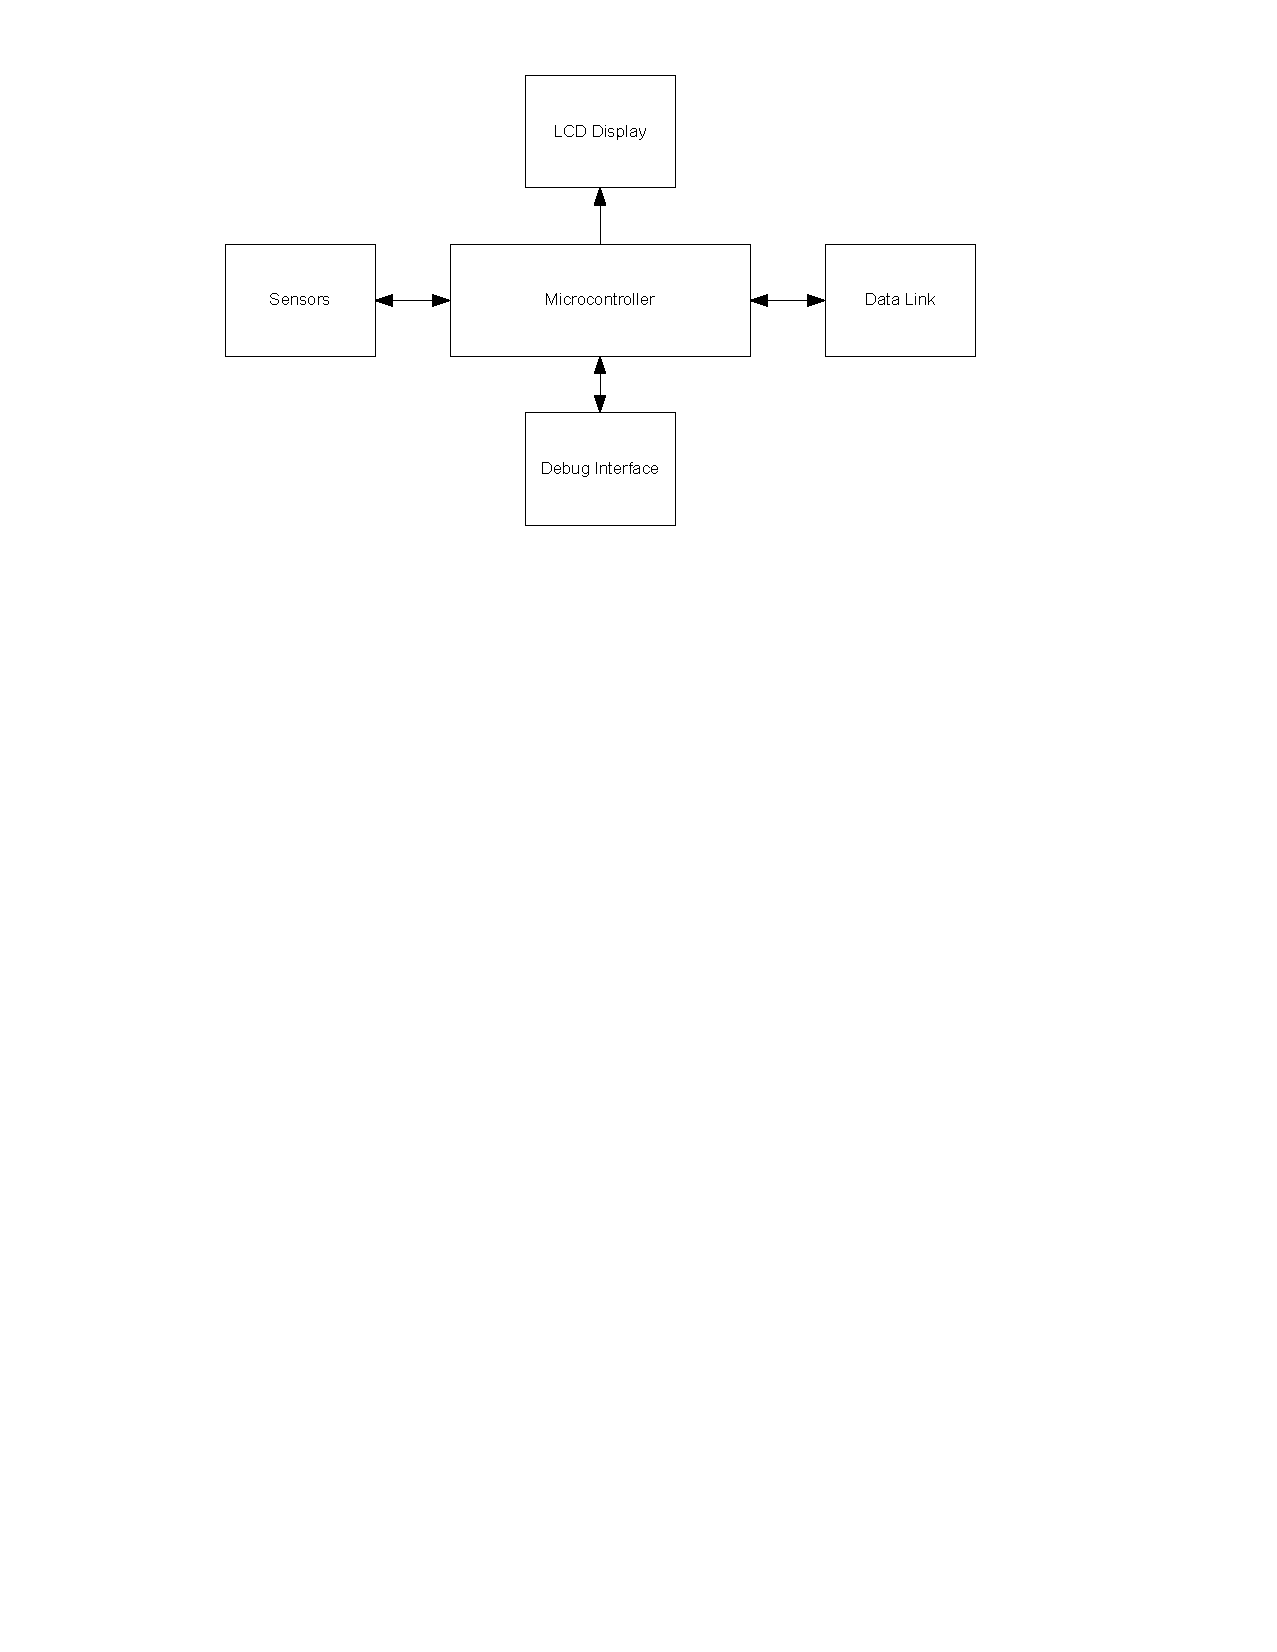
\includegraphics[width=4in]{includes/Simplified_MSP430}
\caption{A simple hardware block diagram of the PICA E-Meter.}
\label{fig:simple_e_meter_diagram}
\end{center}
\end{figure}
This block diagram describes 5 major subsections of the E-Meter, the microcontroller, the \ac{LCD} screen, the sensors, the data-link, and the debug interface. In order to construct a fully working E-Meter each of these components required some individual proving and then integration into the final design.

\subsubsection{Microprocessor Integration}
Before beginning work on any of the other components, Team PICA needed to prove that code could be compiled and loaded onto the MSP430 platform. In order to accomplish these two tasks several options exist:
\begin{enumerate}
\item IAR Workbench
\item Code Composer Studio
\item MSPGCC 4.x
\end{enumerate}
The first two options, both provided by \ac{TI}, are proprietary development environments tailored for compiling and debugging embedded C. However, both of these tools are provided for Microsoft Windows only. That being the case, the team wanted to try and work with the open-source MSPGCC4 project as the compiler and debugger could run on any computing platform. At the time this seemed like a good idea as the two team-members working on the E-Meter did not use Microsoft Windows as their primary computing platform.

After some configuration, the team successfully compiled and installed the MSPGCC compiler. A full guide to repeating this process can be found in appendix \ref{sec:mspgcc4_ubuntu}. The first test, after setting up the toolchain, consisted of determining if the computer could detect and properly configure the MSP430 programming pod. Figure \ref{fig:msp430_programming_pod_detection} shows the dmesg output showing successful pod detection and configuration.
\begin{figure}[htbp]
\begin{center}
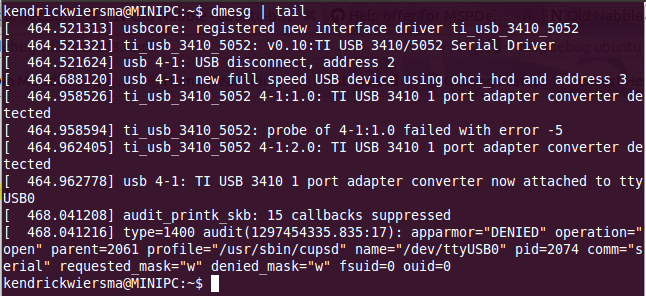
\includegraphics[width=5in]{includes/MSPGCC_Detect_Pod}
\caption{Dmesg output showing Ubuntu Linux correctly detecting and configuring the MSP430 programming pod.}
\label{fig:msp430_programming_pod_detection}                                            
\end{center}
\end{figure}
At this point, the programming pod is recognized as a valid USB device and configured, thus the pod can configure the MSP430 device. However, at this point the team learned that while the MSPGCC4 toolchain supported their device, the debug utility, mspdebug did not support loading code through the team's programming pod. Thus, while MSPGCC4 could compile code, the team would need another tool to load compiled code onto the microprocessor.

Upon learning that MSPGCC4 would not work, Team PICA turned to the suggested tool for developing MSP430 software, IAR Workbench. However, after several trial runs, the team readily switched to \ac{CCS4} for its advanced debugging abilities and familiar interface (Code Composer Studio is based on the Eclipse platform). The version of IAR workbench provided with the MSP430 development kit allowed the user to step through either C code or the translated Assembly instructions, but did not allow the user to view that status of the internal registers.

Using \ac{CCS4} team PICA wrote a ``Hello World'' program for the MSP430, capable of blinking one of the onboard \acp{LED}. This provided conclusive evidence that the team could successfully write, compile, load, execute, and debug code for the MSP430. See appendix \ref{sec:hello_world} for a listing of our ``Hello World'' program.

\subsubsection{LCD Integration}
Team PICA decided to begin integration of external peripherals with the \ac{LCD} as SynchroSystems had already provided driver software compatible with the MSP430 family of devices. After some minor tweaking to tailor their provided driver and demo to run on the MSP430F47197, the design team could successfully compile code to work with the \ac{LCD} screen. Primarily this tailoring consisted of porting their code to use the LCD\_A controller (an integrated peripheral on the MSP430F47197) as opposed to the \ac{LCD} Controller found on some of the other MSP430 devices. However, simply porting the driver did not address the physical hardware connection of adding a screen to the MSP-TS430PZ100A development board donated by \ac{TI}.

In order to make the physical connection between the SynchroSystems SCLCD and the MSP-TS430PZ100A (hereafter refered to as MSP430 development board) Team PICA designed a breakout board using the freely available EAGLE schematic and \ac{PCB} layout software. See figure \ref{fig:sclcd_breakout_board} for a picture of the \ac{CAD} drawing of the breaout board.
\begin{figure}[htbp]
\begin{center}
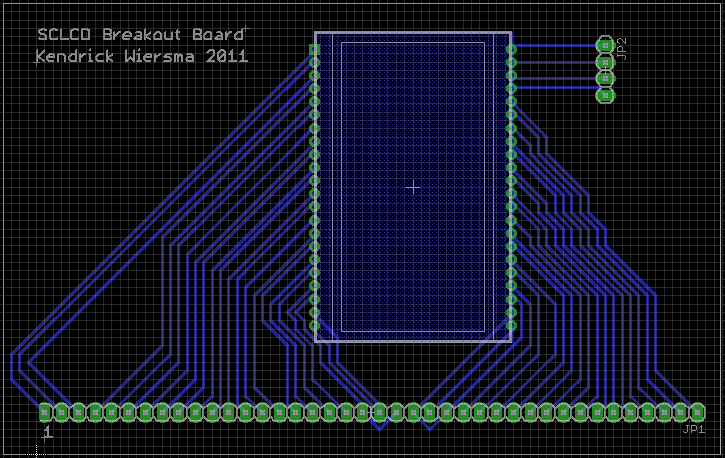
\includegraphics[width=5in]{includes/SCLCD_Breakout_Board}
\caption{EAGLE \ac{CAD} drawing of the SCLCD Breakout Board.}
\label{fig:sclcd_breakout_board}
\end{center}
\end{figure}
After correspondance with Chuck Cox, owner of SynchroSystems, SynchroSystems provided an EAGLE library containing the \ac{CAD} drawings of their part, allowing the breakout board to be produced quicker. At the time of this writting this part library is not available for public release.

During the \ac{LCD} integration testing, Team PICA discovered that the MSP430 peripherals did not operate in the same clock domain as the microprocessor core. Thus, while the core worked properly via the \ac{JTAG} pod, the peripherals did not receive any clock signal. After reading through the user's manual \cite{MSP-TS430PZ100A_users_guide}, the team learned that the MSP430F47197 microprocessor required an additional clock circuit to drive the peripherals, which operate at a different frequency than the main processor. The clock circuit can be seen in figure \ref{fig:msp430_aclk}. This clock operates at $32.768\kilo\hertz$, and from it the MSP430 derives the signal known as ACLK.

\begin{figure}[htbp]
\begin{center}
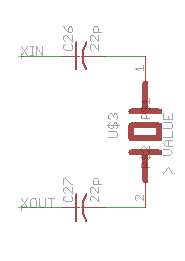
\includegraphics[height=2in]{includes/emeterhw/aclk_crystal}
\caption{32.768MHz clock circuit for MSP430 development board.}
\label{fig:msp430_aclk}
\end{center}
\end{figure}

With the addition of this clocking circuit, and a 22uF capacitor on the LCDREF pin, the \ac{LCD} screen immediately began displaying characters and the modified demo from SynchroSystems ran properly. A video of the \ac{LCD} screen working can be seen at \url{http://youtu.be/9oDglYHUhxo?hd=1}.

\subsubsection{Current Sense Integration}
After Team PICA had the ability to display data on a local \ac{LCD}, the next logical step becomes to collect data from our sensors. As previously noted, the MSP430F47197 contains seven 16-bit Sigma-Delta (abbreviated SD16) \ac{ADC}s used to convert a voltage into a digital measurement. For either our 3-phase or our 1-phase configuration, each SD16 converter used requires an input network to ensure that the differential voltage applied to the terminals of the \ac{ADC} does not exceed $500\milli\volt$. As the team decided to demonstrate 3-phase metering in its prototype, that configuration will be used as an example.

In order to verify that the current sense input network would function as specified, the team ran simulations in LTSpice IV. Figure \ref{fig:current_sense_ltspice} shows the LTSpice schematic for the current sense network, while figure \ref{fig:current_sense_ltspice_trace} shows the final test output.
\begin{figure}[htbp]
  \centering
  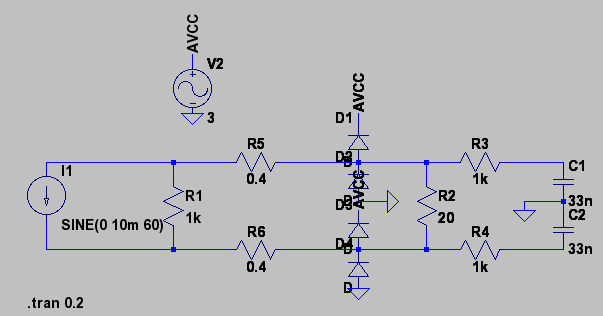
\includegraphics[width=5in]{includes/emeterhw/current_sense_ltspice}
  \caption{Current sense input network verification using LTSpice.}
  \label{fig:current_sense_ltspice}
\end{figure}
\begin{figure}[htbp]
  \centering
  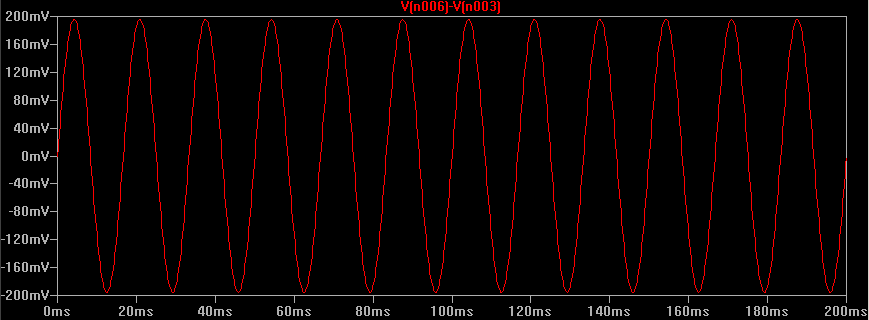
\includegraphics[width=5in]{includes/emeterhw/current_sense_ltspice_trace}
  \caption{Results from the LTSpice verification of the current sense input network.}
  \label{fig:current_sense_ltspice_trace}
\end{figure}
This particular input board design covers $10\ampere$ circuits, as such, in the worst possible scenario the current transformer can produce $10\milli\ampere$ when $10\ampere$ conducts on the main lines. A current source in figure \ref{fig:current_sense_ltspice} represents the current transformer output. The results then show that when measuing maximum line current flow, the differential output of the current sense network remains at approximately $400\milli\volt$, as seen in figure \ref{fig:current_sense_ltspice_trace}. This test ignores the varistor, as the LTSpice model behaves poorly and it exists for extreme cases. Diodes D1 through D2, in figure \ref{fig:current_sense_ltspice}, provide clamping, should some part of the input network fail, and exceed the maximum rating of the circuit.

Of the seven available SD16 converters, two are dedicated to each phase of the power. The first SD16 for each phase measures the current, using an input network seen in figure \ref{fig:sd16_current_sense_input}.
\begin{figure}[htbp]
\begin{center}
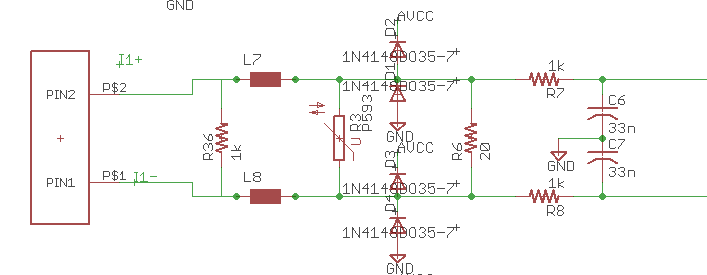
\includegraphics[width=6in]{includes/emeterhw/current_sense_eagle_schem}
\caption{SD16 current sense input network.}
\label{fig:sd16_current_sense_input}
\end{center}
\end{figure}
The positive and negative terminals of a current transformer attach to points PIN1 and PIN (as seen in figure \ref{fig:sd16_current_sense_input}) in the SD16 input network. A current transformer provides a convenient method for measuring large currents by keeping the wires carrying large currents physically detached from the circuit. Current transformers rely on a process known as induction, where a wire carrying current is passed through a loop, or many loops, of wire. Those loops of wire then begin to conduct current in response to the \ac{EM} field produced by the current carrying wire. The input network can sense the wire-loop's induced current as a differential voltage, which the SD16 can then convert into a digital measurement. The inductors, L1 and L2 provide protection against any electro-magnetic interference while the varistor R3 and diodes D1-D4 provide protection against large transient spikes should the current transformer induce too large a current. Resistor R36 is known as the burden resistor for the current transformer, which provides a low impedance path for induced current to flow, and further limiting the amount of induced current in the current transformer, keeping the circuit operating in a stable and predictable manner. Additionally, the burden resistor translates the induced current to a voltage for the reaminder of the circuit. The current transformer datasheet \cite{CST1020} contains a table specifying the burden resistor to produce a desired voltage. The datasheet recommended a $500\ohm$ burden resistor to produce $0.4\volt$ and $2\kilo\ohm$ burdon resistor to produce $0.6\volt$. As the SD16 input differential constaint is $0.5\volt$, we chose a value between those specified on the datasheet, $1\kilo\ohm$ for the burden resistor. The remaining resistors, R7 and R8, along with capacitors C6 and C7, server to further limit and scale the generated differential voltage from the burdon resistor before being read by the SD16 converter. This portion of the circuit comes from a \ac{TI} application note regarding the SD16 input network \cite{slaa409}.

The design team chose to use a relatively small turns ratio current transformer to allow for more headroom on the input network. The CST-1020 used in the prototype has a turns ratio of 1:1000, meaning there are 1000 turns for every one turn of wire passing through the center. For the prototype, where our meter would not be reading more than $20\ampere$, the limit of these current transformers, this would provide us with a maximum of $20\milli\ampere$ of induced current. For a production design, the current transformers would be required to read currents of up to $200\ampere$ or more, requiring that the current transformer be resized to 1:10000 or greater. However, as large turn ratio current transformers tend to be costly, the team chose to use the more cost effective, lower turns ratio current transformers for the proof-of-concept E-Meter prototype.

Once the design team added the serial data port, discussed in the next section, the upper four bits of the data could be transmitted back to the workstation \ac{PC} for processing in MATLAB. While the SD16 converter measures 16-bit voltages, the serial port can only transmit 8-bit characters, only some of which are printing characters. By truncating the measurements to four bits, the values could be added to a reference character (uppercase 'A') to map the values 0 through 15 into the characters 'A' through 'P'. As the intent of this test was to verify that readings from the SD16 were periodic in nature, four bits of low-resolution could still satisfy the goal. By showing that the SD16 converter could properly capture and read a periodic waveform the team proved that the SD16 converter functions as expected. See figure \ref{fig:4bit_current_sense} for the test results.
\begin{figure}[htbp]
\begin{center}
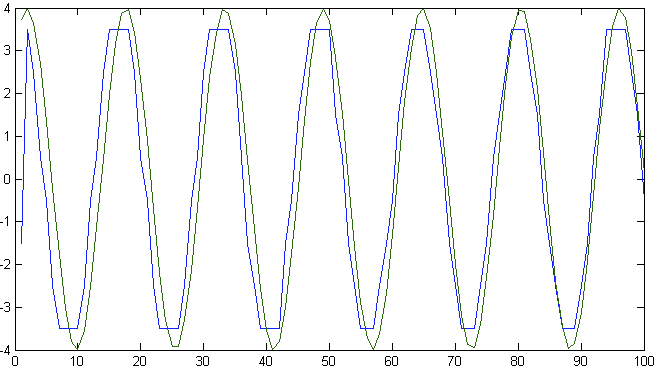
\includegraphics[width=5in]{includes/4bit_current}
\caption{Data captured from the SD16 converter over RS232 (blue). Ideal sinusoid (green).}
\label{fig:4bit_current_sense}
\end{center}
\end{figure}
The results really need very little explanation, figure \ref{fig:4bit_current_sense} shows that the output of the SD16 converter, once normalized to zero, can properly read a sinusoid. Given that only the top 4 bits of the result were captured for this test, the resolution of these readings dropped significatly: the extreme values of the sinusoids are not represented, as this four-bit system does not provide enough resolution to distinguish them from the neighboring values. Restoring more of the 16-bit resolution by keeping more bits would help relieve this issue. See appendix \ref{sec:sd16_to_uart} for the code used in this test.

\subsubsection{Voltage Shunt Integration}
In addition to measuring current, the PICA E-Meter must also collect data about the line voltage. While three of the 7 Signal-Delta \acp{ADC} are used for current measurements, the next three are used for voltage measurements when in the 3-phase configuration. Again, the SD16 converters only allow a $500\milli\volt$ differential input, so the team designed an input network to step down the 120VAC to a safe level to input into the converters. This circuit comes almost entirely from a \ac{TI} application note regarding using the MSP430 for 3-phase power monitoring \cite{slaa409} and can be seen in figure \ref{fig:voltage_shunt_input_network}.

\begin{figure}[htbp]
  \centering
  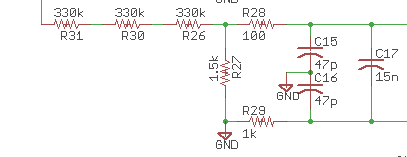
\includegraphics[width=5in]{includes/emeterhw/voltage_shunt_eagle_schem}
  \caption{Voltage shunt input network.}
  \label{fig:voltage_shunt_input_network}
\end{figure}

In order to verify that the circuit worked as expected, LTSpice IV was used to simulate a 120VAC signal entering the network. The schematic for this simulation can be seen in figure \ref{fig:voltage_shunt_ltspice} and the results in figure \ref{fig:voltage_shunt_trace}.
\begin{figure}[htbp]
  \centering
  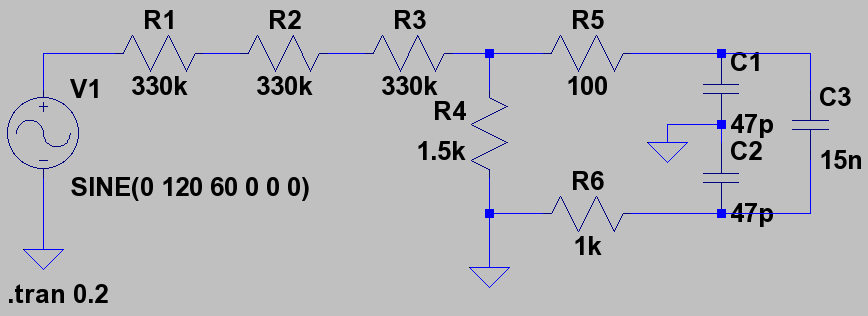
\includegraphics[width=5in]{includes/emeterhw/voltage_shunt_ltspice}
  \caption{Voltage shunt input verification using LTSpice.}
  \label{fig:voltage_shunt_ltspice}
\end{figure}

\begin{figure}[htbp]
  \centering
  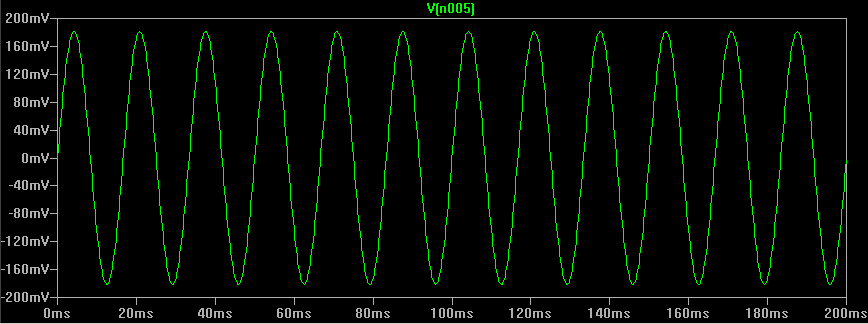
\includegraphics[width=5in]{includes/emeterhw/voltage_shunt_trace}
  \caption{Results from LTSpice verification of voltage shunt input network.}
  \label{fig:voltage_shunt_trace}
\end{figure}
Figure \ref{fig:voltage_shunt_trace} shows a peak-to-peak measurement of approximately $330\milli\volt$, which is within the required range for the SD16 converter. Measurements taken of the realized circuit indicate approximately a $355\milli\volt$ differential voltage which is within the component tolerance of 5\%.
\begin{align}
330\milli\volt \times 0.05 &= 16.5\milli\volt\\
16.5\milli\volt \times 2 &= 33\milli\volt\ \mathrm{peak-to-peak}\\
330\milli\volt + 33\milli\volt &= 363\milli\volt < 500\milli\volt
\end{align}

Like the previous sensor integration test, upon first attaching the voltage shunt network, the top four bits of the converted result were transmitted back over the \ac{RS232} uart. This data could then be processed by MATLAB and plotted. The results are seen in figure \ref{fig:4_bit_voltage_shunt}. The data captured looks very corse and lacks the precision necessary for an E-Meter to properly calculate the power used. The team expects that by finding a method to transmit all 16 bits back, as opposed to only the truncated top four bits, the precision of the results will increase.

\begin{figure}[htbp]
  \centering
  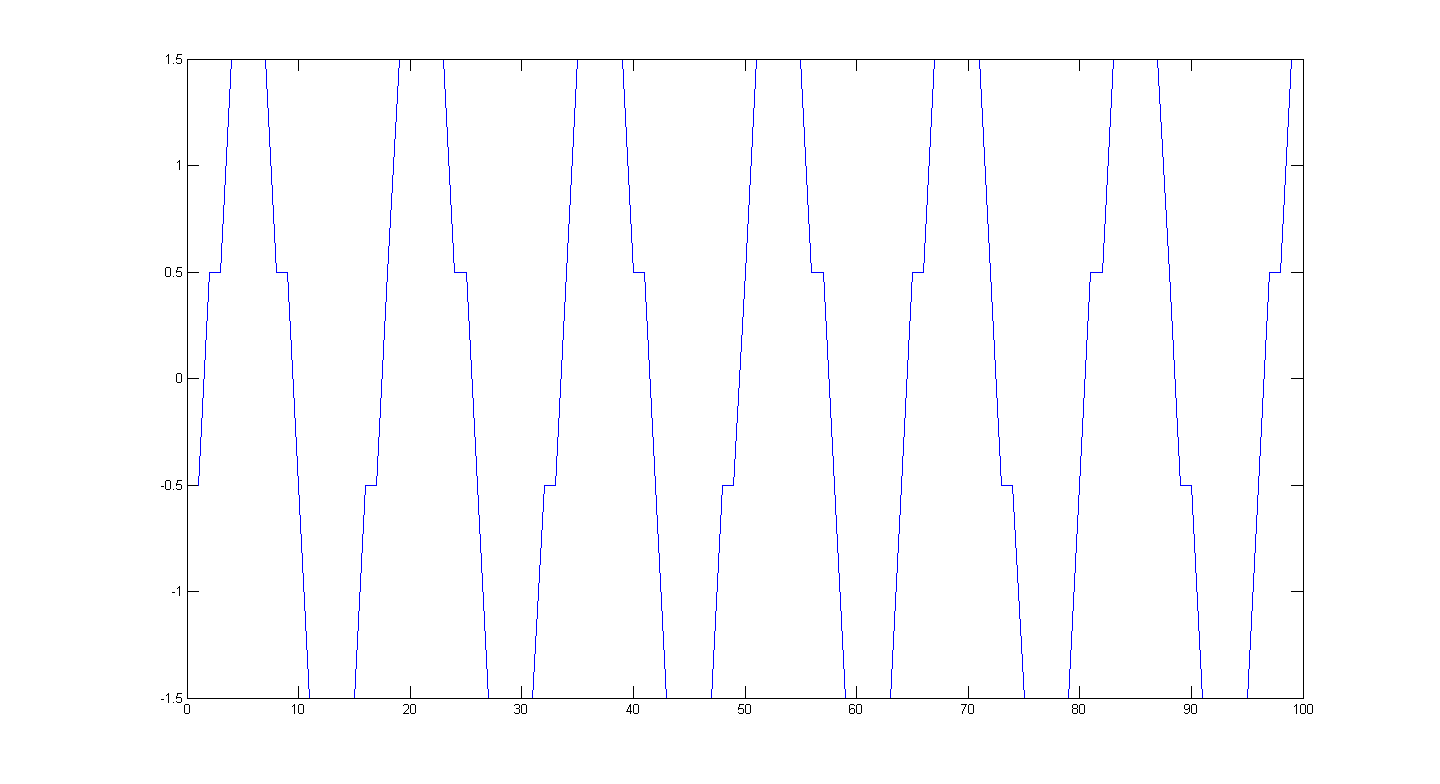
\includegraphics[width=5in]{includes/4bit_voltage}
  \caption{Voltage data captured from the SD16 converter over RS232.}
  \label{fig:4_bit_voltage_shunt}
\end{figure}
  
\subsubsection{Serial Data Link Integration}
The second to last block of the block diagram in figure \ref{fig:simple_e_meter_diagram}, data link, describes the method for communicating the measured data to the rest of the world. Ultimately, Team PICA desires to implement an Xbee radio communication system, however, before using the Xbee radio a simple RS232 \ac{UART} fulfills the data transmission requirement. By first implementing a simply prototype, \ac{RS232}, the team could begin development with some basic functionality before moving onto integrating the more sophisticated wireless Xbee. Additionally, if serial communications functions properly, making the change to Xbee is trivial, as the Xbee radio uses a serial RS232 based interface.

In order to implement RS232 communication the design team chose to use the MAX233A \ac{IC} which comes in a 20-pin \ac{DIP}. The MAX233A provides line-level conversion from the $3.0\volt$ output of the MSP430 up to the $5.5\volt$ required for RS232 communication. Conversely, the chip also converts the receive line from RS232 $5.5\volt$ down to $3.0\volt$ for the MSP430 \ac{UART}. Other methods exist for performing this line-level conversion, however the MAX233A provides a simple, 1-chip solution without requiring large amounts of board space and without adding significant cost to the final product. See figure \ref{fig:max233a_serial_data_link} for the serial data-link circuit used in the PICA E-Meter. Any number of the MAX23X devices could have been used for this purpose, however the MAX233A required the least number of external components. Without an integrated solution, the team could have designed a circuit using optocouplers and transistors to mimick the functionality (stepping up and down the RS232 voltages), however this method would require 6 discrete components, totaling a space larger than the MAX233A \ac{IC}.
\begin{figure}[htbp]
\begin{center}
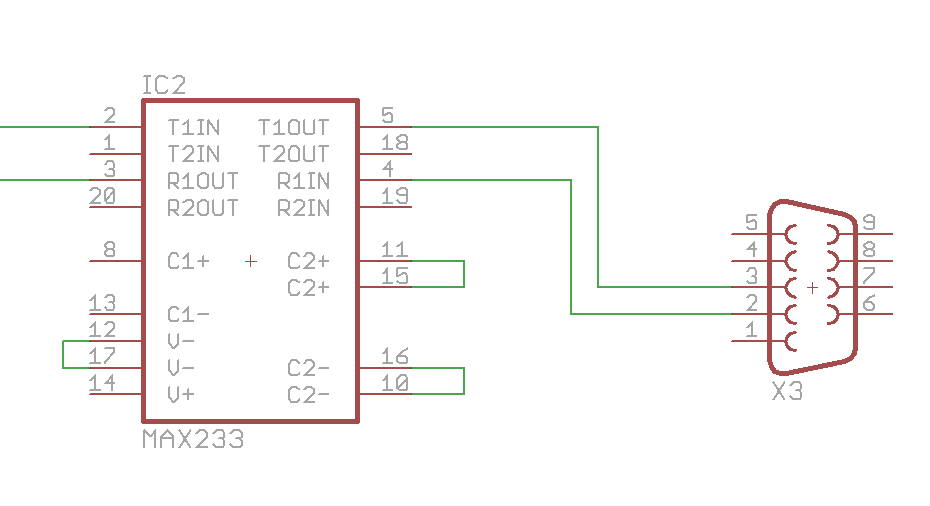
\includegraphics[width=5in]{includes/max233a_circuit}
\caption{MAX233A RS232 serial data link circuit.}
\label{fig:max233a_serial_data_link}
\end{center}
\end{figure}

In order to verify the proper operation of the serial data link, the team performed an echo test. Code running on the MSP430 receives a character from the receive buffer and simply moves it to the transmit buffer on a receive interrupt. Characters typed into a serial terminal on the team's workstation \ac{PC} would then be transmitted from the computer, to the MSP430 before being transmitted back to the PC and displayed in the terminal window. This operation succeeded on the very first attempt with the results seen in figure \ref{fig:rs232_echo_register} and \ref{fig:rs232_echo_terminal}.
\begin{figure}[htbp]
\begin{center}
\subfloat[Serial \ac{UART} registers in the MSP430]{\label{fig:rs232_echo_register}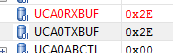
\includegraphics[width=2in]{includes/rs232_echo_registers}}\quad
\subfloat[Serial \ac{UART} terminal on the workstation \ac{PC}]{\label{fig:rs232_echo_terminal}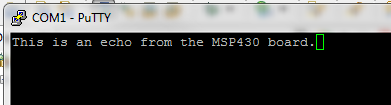
\includegraphics[width=3in]{includes/rs232_echo_terminal}}
\caption{RS232 Echo Test}
\label{fig:rs232_echo_test}
\end{center}
\end{figure}
Even though serial communication provides basic data transmission, the team desired to implement a wireless interface to the E-Meter, allowing for greater distance between the unit and the data recipient. The original target, Xbee radio, uses a serial interface, essentially making it a wireless \ac{RS232} cable. Each Xbee device holds non-volatile configuration data describing the devices function, either an end-device or a router. The Xbee devices, however, require an additional signal, \ac{DTR}, to alert the device when a data packet is ready for transmission. The MSP430 software will need to generate this signal when it wants to transmit data.

During testing with the Xbee radio the team added support for flow control to the RS232 port to better control the transmission timing of the Xbee devices. This simply involves adding two additional signals between the D-Sub 9 connector and the MAX233A chip, along with two additional lines to the MSP430. As of right now, software support for flow control does not exist. See figure \ref{fig:rs232_flow} for a full schematic for the \ac{RS232} connection.
\begin{figure}[htbp]
  \centering
  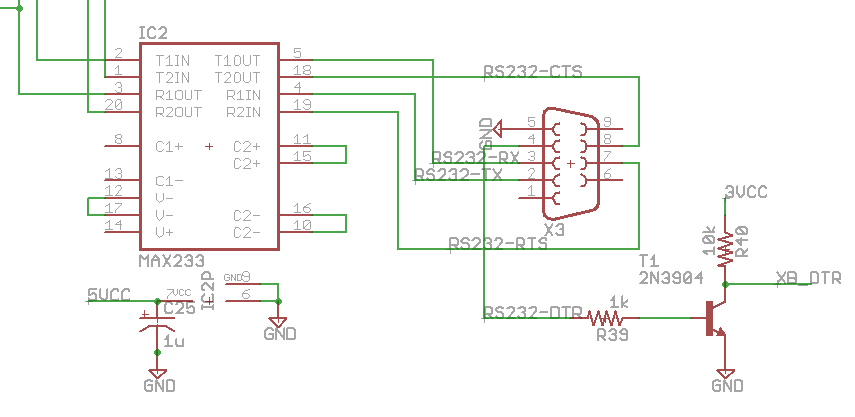
\includegraphics[width=4in]{includes/Complete_RS232_DTR}
  \caption{Flow control and DTR lines for RS232 communications}
  \label{fig:rs232_flow}
\end{figure}

\subsubsection{Debug Interface Integration}
In order to properly load software onto the MSP430, the team needed to implement a \ac{JTAG} port in the final design of the prototype. The \ac{JTAG} standard defines the implementation of the communications protocol as well as circuitry needed to interface a \ac{JTAG} programmer and the \ac{JTAG} port on a device. For the E-Meter, see figure \ref{fig:jtag_circuit} for the \ac{JTAG} interface circuit. \ac{TI} has chosen to use a 14-pin interface for its \ac{JTAG} devices. Additionally figure \ref{fig:jtag_circuit} shows the pin header (SV1) that allows the source of the $3\volt$ supply to change between an external power supply and the internal \ac{JTAG} pod power.
\begin{figure}[htbp]
\begin{center}
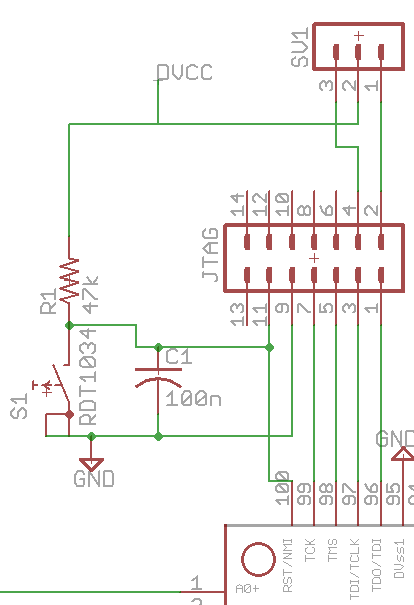
\includegraphics[height=4in]{includes/JTAG_Circuit}
\caption{\ac{JTAG} circuit for the MSP430F47197.}
\label{fig:jtag_circuit}
\end{center}
\end{figure}
In a final production version the \ac{JTAG} interface must remain on the \ac{PCB} for the initial programming of the microprocessor and allowing for software reset. However, the 14-pin header should not be populated on the \ac{PCB} making it more difficult for the end-user to reprogram the meter, or read out proprietary firmware.

In order for \ac{JTAG} to properly configure a device, four signals must be present, with an optional fifth signal:
\begin{enumerate}
\item TDI: Test Data In
\item TDO: Test Data Out
\item TCK: Test Clock
\item TMS: Test Mode Select
\item TRST: Test Reset (optional)
\end{enumerate}
The MSPP430 processor has dedicated ports for each of these signals which arrive through the \ac{TI} programming pod. In order to add this functionality to the E-Meter \ac{PCB}, a 14-pin header provides the interface between the programming pod and the microprocessor. The signals can either be hardwired into the microprocessor, or as seen in figure \ref{fig:jtag_circuit} with minimal extra circuitry, allow for a push-button reset switch. Effectively, this switch drops the VCC to ground, killing power to the microprocessor, and pulsing the \ac{TRST} line, which halts activity. Because the programming pod provides capability to power the microprocessor, and additional header allows for switching between the programmer power and the board power. Capacitor C1 in figure \ref{fig:jtag_circuit} simply provides debouncing on the incoming signal. This prevents cases where the user depresses the buttons incompletely, potentially causing several partial resets.


%\subsection{Software Design}
%The design team chose to use embedded C to implement the software for the PICA E-Meter. \ac{TI} provides header files to aid writting embedded C code, and although these headers can also be used in assembly programming, using embedded C greatly improves the readability of the code for the designers.
% E-meter software design, by Avery
\subsection{Software Design}

The typical programming paradigm for the MS430 is to
maximize the amount of time the processor spends in the sleep
state. To do this, many of the peripherals on the MS430 chip can be
configured to generate interrupts that wake the processor and execute
code relevant to the triggering events. The software designed for the
E-meter follows this paradigm of sleeping and interrupts, as pictured
in \ref{fig:emeter_software_flow}.

\begin{figure}[htbp]
\begin{center}
  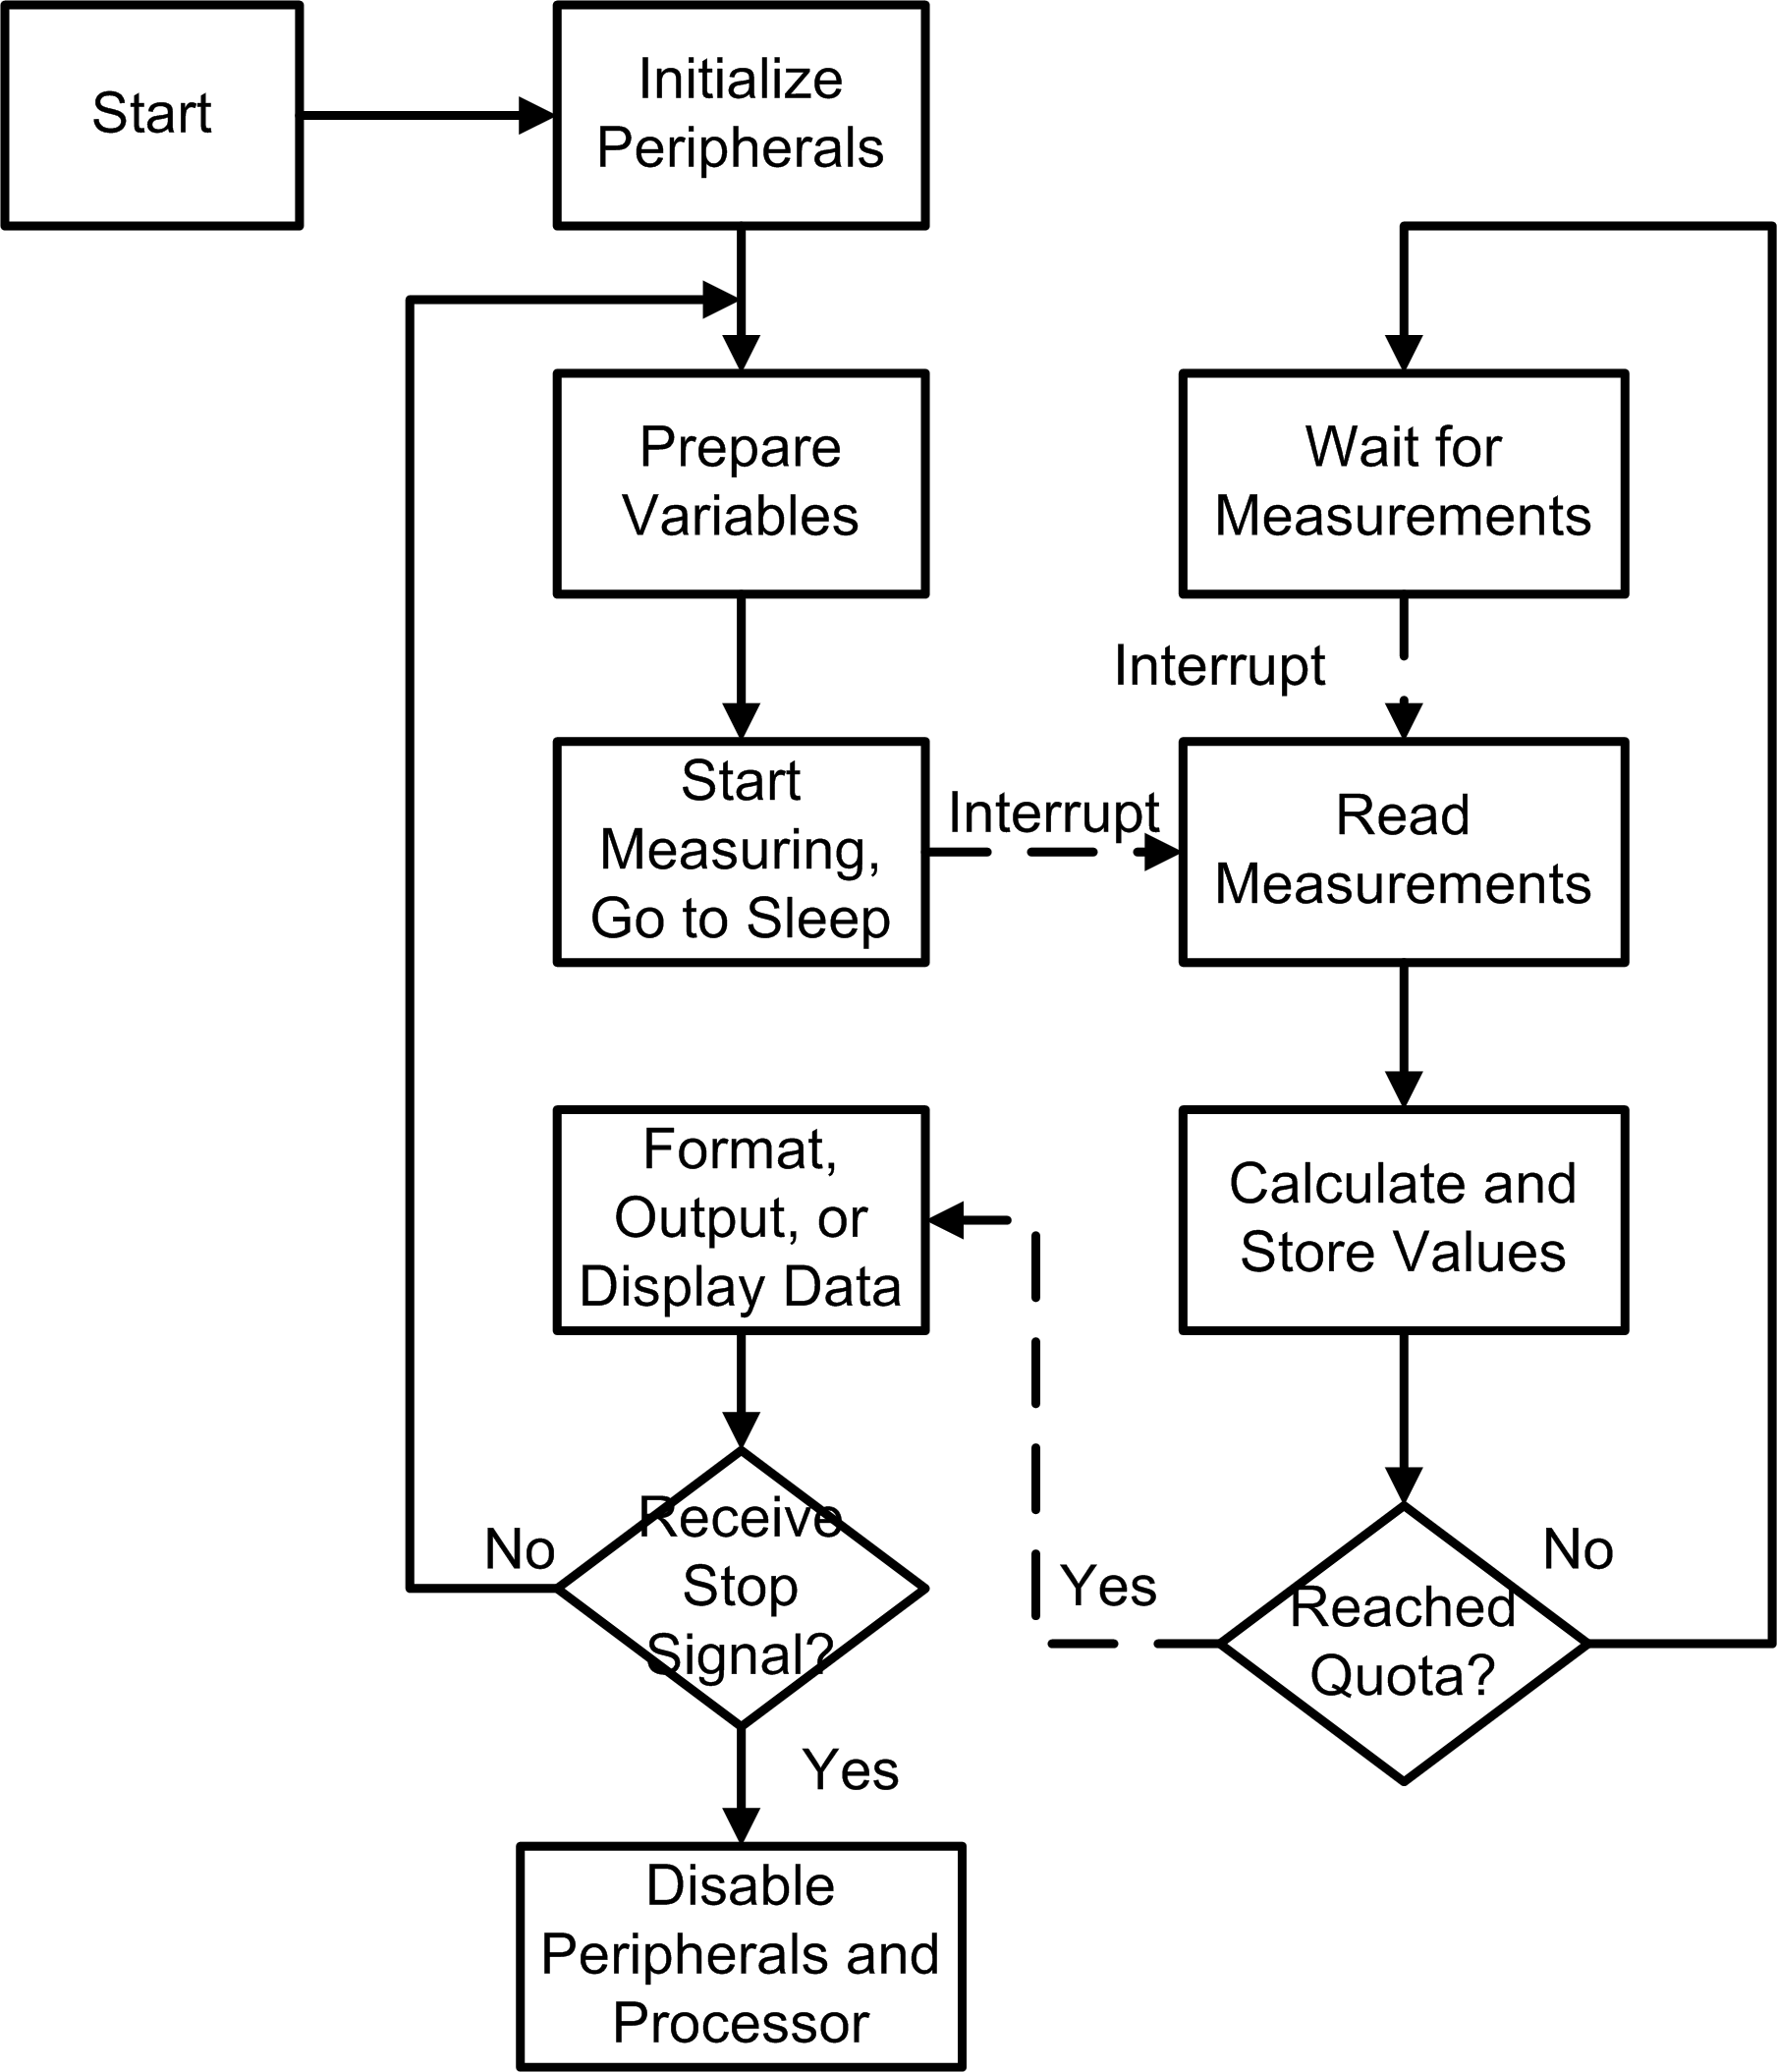
\includegraphics[width=5in]{includes/Emeter_Software_Flowchart}
  \caption{E-Meter Software Flow Diagram}
  \label{fig:emeter_software_flow}
\end{center}
\end{figure}

\subsubsection{Design}
The primary focus of the E-meter is measuring the current load and
line voltage of each phase of electricity entering the building. The
input networks for the E-meter convert these different elements into
voltages that the MSP430 can read on its dedicated \ac{ADC}
hardware. The E-meter software must allow time for these \acp{ADC} to
resolve the voltages, but must also output summaries of these
measurements to its built-in LCD screen and to the base station. To do
this, the software running in the E-meter first loads pre-defined
values into the device's configuration registers, then measures the
voltages on the \acp{ADC}, outputs a summary of the information
collected, then repeats the collection and output sections. For
simplicity, the conversion factors to map these values ranging from
$-0x8000$ to $0x7999$ into their real-world values (such as $\pm
120\sqrt{2}\volt$) are hard-coded into the program at compile time
using several \texttt{\#define} statements.

The initialization step loads values into the MSP430's configuration
registers that enable the desired features of the E-meter. The list of
possible values can be found in the MSP430 User Manual\cite{slau056j},
which design team referenced frequently in determining the values for a 
suitable configuration. In the current version of the software, the
first six \ac{ADC} channels are ``grouped'' together while the seventh is
disabled. Grouping the channels ensures that all six will measure at
the same time, and will only generate one interrupt that signals when
all six have finished measuring. The \acp{ADC} measure voltages
between $-0.6 \volt$ and $0.6 \volt$ and returns 16-bit
two's-complement integers that represent that range. The \ac{IEEE} 754
standard requires a 32-bit floating point number to have at least 23
binary places of precision, which could store several of these
readings without roundoff error. Additionally, the setup stage selects
the clocking frequency for the \acp{ADC} and for the serial \ac{UART},
selects which of the \acp{ADC} to measure, and which pins are used for
the \ac{LCD} display.

As the final task in this preparation stage, the program
enters a loop where the main calculations take place. At the beginning
of this loop, the processor enables the \acp{ADC} and puts the main
process to sleep.

When the \acp{ADC} have measured the voltage from their attached
circuits, the ``group leader'' may raises an interrupt to signal the
completion of the measurement. This interrupt triggers the \ac{ADC}
\ac{ISR}, which checks that the \ac{ISR} was indeed caused by one of
the active \acp{ADC}. After doing so, the \ac{ISR} turns off
the \acp{ADC}, preventing the \acp{ADC} from interrupting again before
the original interrupt can be cleared. the \ac{ISR} then reads the
volage and current for the first phase. It uses the hardware
multiplier to square the 16-bit-integer current and voltage
measurements into 32-bit square measurements, and also computes the
instantaneous power by multiplying the current by the voltage. Each of
these 32-bit integers are then summed with a corresponding 32-bit
floating-point number, a process which takes a considerable amount of
computation but allows for much larger numbers to be
represented. This is essential for computing RMS: in order to find the
mean of the squares, the squares must be summed together without
exceeding the limits on their representation. 32-bit \ac{IEEE} floating-point
numbers can express numbers up to $2^{127}$, which is many orders
greater than the $2^{31}$ limit on integers; hence, using
floating-point numbers for storing sums prevents overflow when a
limited number of sums are to be stored. The program defines a quota
for the number of samples to take before computing the mean and
outputting data. This limit means that a known number of items will be
summed, which not only prevents overflow but also ensures that the
output from the E-meter will occur at regular intervals. While a timer
could provide the desired regularity, connecting the output rate to
the measurement rate gives an implicit indication of the measurement
rate without requiring special debugging equipment.

In contrast with resetting the processor, waking the main process
resumes execution at the same location where it went to sleep. With
the newly-measured sum-of-squares for current and voltage for all
three channels, as well as the sum of instantaneous power during the
sampling period, the main process decides what it needs to calculate
for output. In the current version of the software, the E-meter
transmits power of all three phases and total power for each run
through the main loop; unless the \ac{LCD} screen displays current or
voltage, their \ac{RMS} values are unneeded. The main loop always
calculates power and energy consumed for output and accumulation,
respectively.

If necessary, the loop continues the computation of \ac{RMS} voltage
and current by first finding the mean of the squares by dividing the
sum of the squares by the number of measurements, then calculates the
square root of these mean squares, thereby giving the RMS measurement;
multiplying by the callibration factors gives the real-world voltage
or current. These values are then output to the LCD screen, as
detailed in the 

As the power is not measured by squaring, the power sum is simply
divided by the number of measurements to obtain the mean real power;
the energy total is incremented by the product of the power and the
time taken to perform the measurements and calculations, which one of
the timers tracks. By applying the callibrated conversion factors,
the software computes power in watts and the acculated power in
watt-hours. 

\subsubsection{User Interface}
In lieu of a working XBee network, the primary interface to the
E-meter uses the single touch-button and the \ac{LCD} screen. The LCD
display uses the four digit places in the upper-right corner to
display the current uptime in hours and minutes. The center dial
displays the seconds elapsed: every five seconds, another of its
twelve regions fills, until it resets at the end of each minute. The
upper-left characters indicate which of power, energy, current, or
voltage is displayed. The actual value is displayed in the six primary
characters.

The six primary characters show the real-time reading of the selected
value. The first character only indicates the sign of the number: it
is empty for positive values and shows a negative sign when the value
is negative. The next three characters display the value in one of two
forms: either a number from 10 to 999, or a decimal number less than
10 with two following decimal places. The software automatically
determines in which \ac{SI} range to place the value to fit these
forms. The fifth character displays this range: at the moment, this
will be one of ``k'', ``m'', or ``u'' for the prefixes kilo-, milli-,
and micro-, respectively; the space is blank if there is no
prefix. The final character shows the base unit of the measurement:
``A'' for current in amps, ``V'' for voltage in volts, ``W'' for power
in watts, and ``E'' for energy in watt-hours. As there is not enough
room for ``Wh'', ``E'' seemed the next most obvious character to put,
though it may cause confusion if users expect to see only \ac{SI}
units. At present, the power and energy measurements are totals from
all three phases, while the current and voltage read only from the
first phase.

The touch-button will turn on the \ac{LCD} backlight if it has gone to
sleep. If the backlight is on, the button will advance the display to
the next mode. This very simply interface has not been user-tested,
but its simplicity.

\subsubsection{Current Status}
The present software for the E-meter reads the current and voltage
from three separate inputs using six of the seven hardware \ac{ADC}
channels. These channels are grouped together, so they only trigger
the \ac{ISR} when all six have finished measuring. The

At present, the software collects readings from two of the MSP430's
\ac{ADC} ``channels'', simulating what an individual ``phase'' would
be measured. As mentioned in the MSP430 user's guide, these two
channels are grouped together, so they wait for each other to resolve
before triggering the \ac{ISR}. This approach can be extended to the
other channels; with only a few changes in software, all of the six
\acp{ADC} needed for this application can group together.

Laboratory execution and examination using a stopwatch show that the
current software can make approximately 760 measurements per second on
both channels when 120 measurements are taken to compute the \ac{RMS}
data before outputting over RS232.

%\subsubsection{Future Work}
%% We have the LCD and buttons working now
%[software has not yet been designed, however this section will go on to explain the structure of the software. A full listing of the software will eventually be found in the appendix.]



\subsection{Printed Circuit Board}
Team PICA decided for the purposes of this project that a \ac{PCB} would provide the best presentation of the final E-Meter. By designing a \ac{PCB} for the project, the team would gain valuable experience in fabrication, and be able to present a cleaner project. Additionally, a \ac{PCB} can help prevent parasitic capacitance inherent in terminal connections (in particular between the microprocessor and the \ac{LCD}). During the time spent debugging the \ac{LCD} by email with Chuck Cox and John Lupien of SynchroSystems, John mentioned that the stuttering and dim segments seen in our demonstration video could be caused by even a slight extra capacitance. Other components, such as the microprocessor itself, have pins spaced in such a way that a \ac{PCB} becomes a logical method for easily connecting external components.

In order to design the \ac{PCB} the team used the freely available program Eagle, produced by Cadsoft Computer USA. Several versions of the software are available, ranging in price and features from a free board-size limited version to an expensive professional no-limits version. As the team budget did not include software licenses, the free boad-size limited version was used to produce the E-Meter \acs{PCB}. 

Originally the E-Meter would be composed of a single \ac{PCB} containing all of the components except for the power supply. However, as the free version of Eagle only allows for an 80 x 100 mm board, the E-Meter became two linked boards; one for the \ac{ADC} input networks, and the other for the main E-Meter processing and data transmission components. These two boards can be seen in figures \ref{fig:e_meter_main_board} and \ref{fig:e_meter_input_board} (larger versions, and complete schematics, can be found in appendix \ref{sec:e_meter_pcb} and \ref{sec:e_meter_schem} respectively).
\begin{figure}[htbp]
  \centering
  \includegraphics[width=4in]{includes/e_meter_main_board}
  \caption{E-Meter main processing and data transmission board.}
  \label{fig:e_meter_main_board}
\end{figure}
\begin{figure}[htbp]
  \centering
  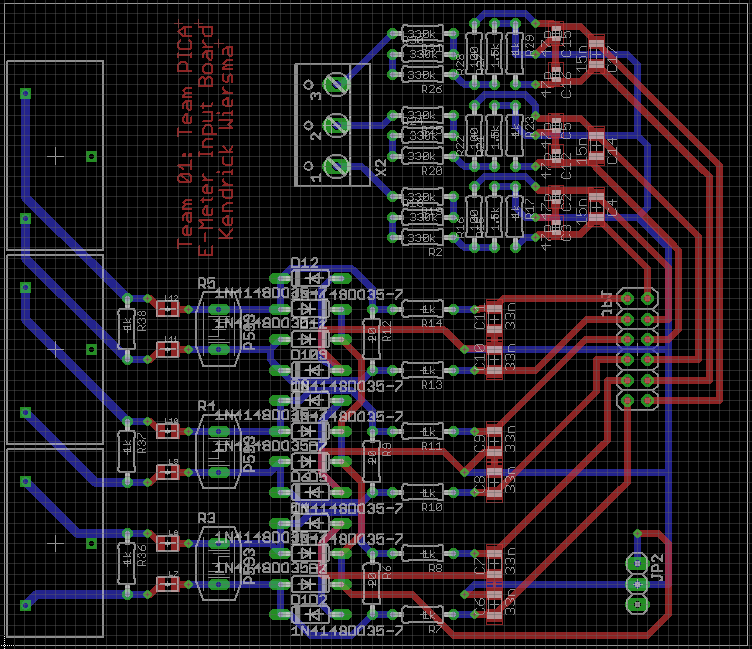
\includegraphics[width=4in]{includes/e_meter_input_board}
  \caption{E-Meter input board.}
  \label{fig:e_meter_input_board}
\end{figure}
Each of these boards are composed of 2 layers, a front and a back. The team chose a two-layer board for several reasons:
\begin{enumerate}
\item The rapid prototype machine, on which \ac{JCI} allowed us to etch our \acp{PCB} only supported two layers.
\item The free version of Eagle only supports creating two-layer boards.
\end{enumerate}
Signals are routed on either side with vias inbetween the two sides. All components are mounted on the top of the board with through-hole components being soldered on the rear.

The main board brings together the \ac{MCU}, \ac{RS232} transceiver, Xbee radio, \ac{LCD}, user pushbuttons, and JTAG interface. Along with these components, several \ac{MCU} peripherals, such as clocks, are also included on this \ac{PCB}. Spatial locality of the components with respect to the \ac{MCU} determined which components appeared on this board, and which components were allocated to the secondary board. Peripherals such as clocks and transmission signals that are susceptible to noise need to be close to the \ac{MCU} to prevent interference from electromagnetic radiation in the environment or the surroundings. In order to further reduce the possibility of electro-magnetic radiation, traces carring signals remain isolated (as much as possible) from traces carrying voltage supply. Where not possible, signal traces were routed between ground traces to provide extra shielding.

Eagle provides part libraries containing \ac{CAD} schematics for many common parts for use in \ac{PCB} development. Many companies also provide custom part libraries with their part to aid designers in during \ac{PCB} layout. For this project, the team used the MSP430 library freely available from \ac{TI} , the SparkFun library, a library from SynchroSystems, and a custom library in addition to the built-in part libraries. Eagle allows users to create custom part \ac{CAD} files to expand the available library of usable components. 

Upon receiving the etched \acp{PCB} from \ac{JCI}, the team verified that the routed traces matched the schematics, and no short circuits were present from mislabeled nets. To check conductivity the team used a \ac{DMM} set to continuity test; placing the leads on connected traces would cause the \ac{DMM} to emit a beep, while non connected traces would result in no sound. After the boards passed verification they were returned to \ac{JCI} to have all surface mount components populated by Joshua Sliter who works in the labs at \ac{JCI} populating prototype boards. The team then added the remainder of the parts. The completed input board and main board can be seen in figures \ref{fig:input_board_assembled} and \ref{fig:main_board_assembled} respectively.

\begin{figure}[htbp]
  \centering
  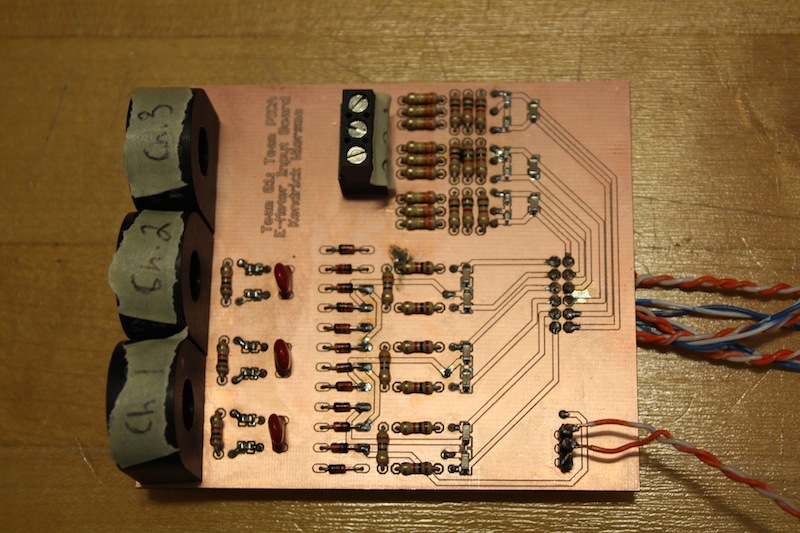
\includegraphics[width=5in]{includes/emeterhw/input_board_assembled}
  \caption{E-Meter input board fully assembled.}
  \label{fig:input_board_assembled}
\end{figure}

\begin{figure}[htbp]
  \centering
  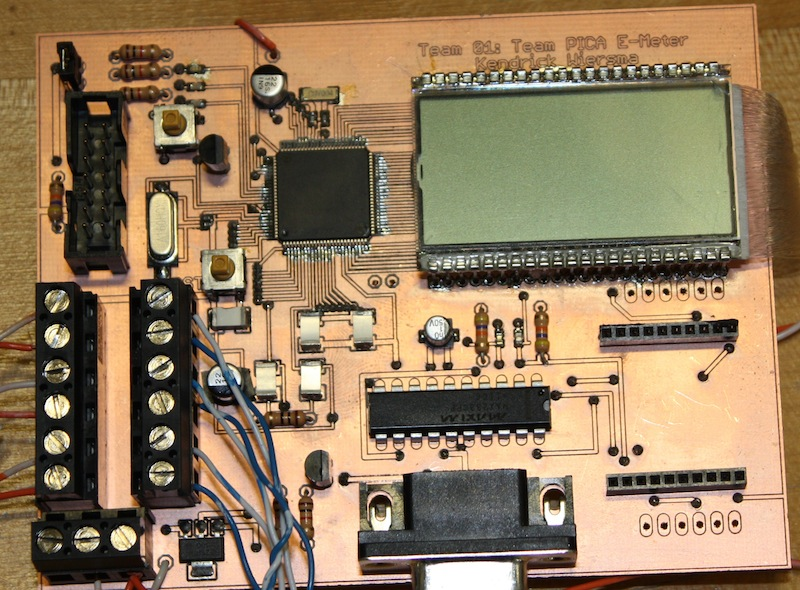
\includegraphics[width=5in]{includes/emeterhw/main_board_assembled}
  \caption{E-Meter main board fully assembled.}
  \label{fig:main_board_assembled}
\end{figure}

%[This section will describe any final implementation details that have not already been covered in the other sections. This may include any mechanical design, such as a case to mount all the parts inside, or any additional hardware such as the power supply. Also included will be several pictures of the completed components.]

\subsection{Testing} % octopus
In order to verify the performance of the PICA E-Meter, several tests stressing various components of the system are described below. These tests verify both functional and behavioral correctness of the E-Meter in various situations, responding to several different stimuli.
\begin{enumerate}
  \item Verify that the connection on the board are reliable. To do this, perform continuity tests on pins that lie on the same \ac{PCB} traces.
  \item Verify that the board contains no ground or board shorts. Perform continuity tests between the ground pin and the signal pins, as well as between the VCC pin and the signal pins. If any are connected, verify that this should be the case.
  \item Verify that the processor can be controlled via \ac{JTAG}. With external voltage applied, attach the \ac{JTAG} pod and re-program the device with the E-meter software by using Code Composer Studio. On the prototype board, removing the RS232 cable increases the success rate of the this procedure.
  \item Verify that the processor can run without the \ac{JTAG} pod. After programming completes, remove the \ac{JTAG} pod and press the reset button. The processor should launch the software automatically. The \ac{LCD} screen should display ``00 W''.
  \item Verify that the SD16s are clocked correctly. The three signal \acp{LED} should display a binary counting-up sequence and the \ac{LCD} screen should show some changes.
  \item Verify that the $32.768\kilo\hertz$ clock is correctly connected by enabling the backlight and waiting for the timeout condition to turn off the backlight.
  \item Verify that the RS232 transmission functions properly by attaching an RS232 cable between the E-Meter and a computer, opening a terminal and verifying that characters are being transmitted.
  \item Verify that the E-Meter is responding to commands via typing the character `q' after performing the previous test. The E-Meter should halt.
  \item Verify that the input board is properly attached to the E-Meter by attaching a load and verifying that the display reads a value within $5\volt$ of $120\volt$.
\end{enumerate}

\subsection{Future Work}

\subsubsection{Hardware}
The prototype of the PICA E-Meter functions properly but it requires several improvements before mass production could begin. First and foremost, the Xbee radio socket does not allow for transmission of data over a wireless link. In fact, the Xbee radio that team PICA first attached to the Xbee socket no longer functions properly when attached to the Xbee developer boards. This observation leads to the natural conclusion that there exists an error in the MSP430 to Xbee interface developed for this project. Likely, the problem lies in the flow control circuitry which did not undergo a full test before being integrated into the final prototype. Secondarily, and potentially related, the \ac{RS232} port on the prototype seems to create issues during the \ac{JTAG} process. Mainly, when attached, the \ac{RS232} cable prohibits the ability to reprogram or debug the MSP430. Team PICA does not fully understand the nature of this particular point of failure, however a simple workaround is to detach the \ac{RS232} during program loading.

A second revision of the E-Meter \ac{PCB} would allow for many of the lessons learned during assembly of the first \ac{PCB} to be incorporated:
\begin{outline}[enumerate]
\1 Plan on soldering the \ac{LCD} to the back of the \ac{PCB}.
\2 In the current design the traces between the MSP430 and the \ac{LCD} are routed on the top of the board, meaning that the \ac{LCD} must be top-soldered to the board.
\2 An unfortunate side-effect of this tweak would be the addition of 40 vias to the back of the board, making the initial assembly more difficult.
\1 Fix the mislabeled net, and attach VCC to the MSP430 processor without the need of a jumper wire.
\2 The first revsion schematic contained a mislabeled net which resulted in having to attach a jumper wire to the prototype \ac{PCB} attaching the $3\volt$ supply to the correct pins of the MSP430 processor.
\1 Move the TX and RX \acp{LED} to the TX and RX lines on the other side of the \ac{RS232} driver.
\2 Currently the TX and RX \acp{LED} are attached between the MSP430 and the MAX233A \ac{RS232} driver \ac{IC}. While the signal will still transmit, the MSP430 cannot drive the \acp{LED} enough to illuminate them.
\2 Moving the \acp{LED} to the other side of the MAX233A driver would allow the higher voltage drive from the \ac{IC} to illuminate the \acp{LED} during transmit/receive activities.
\2 This fix would greatly improve debugging, especially if the \ac{RS232} bug still exists.
\1 Add better labels to components that are sensitive to orientation, reducing the difficulty of populating components to the board.
\1 Ensure that the clocks are surrounded entirely by ground traces, prohibiting the clock signal from leaking into other components on the \ac{PCB}.
\2 While it is not obvious that this problem currently adversely affects any components on the \ac{PCB}, a few small changes would prevent signal leakage.
\1 Move the backlight \ac{LED} to the correct position on the back of the \ac{PCB} underneath the \ac{LCD}.
\2 This removes another small jumper wire used by the team after learning that the backlight fiber-optic lines were not as flexible as previously thought.
\1 Route the $5\volt$ signal from the empty pin on the 3-pin header to the voltage regulator as opposed to using wire jumpers.
\1 Fix the crossed trace on the input board that prevents the second current sense network from operating properly.
\end{outline} 
A second revision of the E-Meter \ac{PCB} would also allow for several enhancements:
\begin{outline}[enumerate]
\1 Additional buttons for a simpler user interface.
\1 Move buttons to more easily accessible position, further simplifying the user interface.
\1 Include space for adding mounting brakets to the \ac{PCB}.
\end{outline}
\subsubsection{Software}
To reduce the impact of noise in the \acp{ADC}, a digital low-pass
filter could be implemented to reject noise in the measurements. In
order to do this, however, the E-meter must be sampling at a rate
high enough to identify higher-frequency fluctuations as distinct from
low-frequency signals like the $60\hertz$ waveform from the \ac{AC}
lines. Insufficient sampling rates would lead to aliasing: signals of
a frequency higher than the sampling frequency would appear as a
low frequency, and would not be rejected. In light of this, the
E-meter software can be optimized in several ways to increase the
sampling frequency.
\begin{enumerate}
  \item Using the \ac{ISR} to read data from the \ac{ADC} registers,
    square and multiply them as usual, then write these values to
    a shared data structure that the main loop can process between
    \ac{ADC} conversions. This approach would require a means to keep
    the \acp{ISR} from overwriting data before the main process can
    read it, but would allow the \ac{ISR} to complete more quickly,
    thereby allowing the \acp{ADC} to perform more conversions.
  \item Creating separate variables for data being read
    and data to display, where the read data is copied to the display
    variables when the display functions have completed. This would
    allow the output loop to run in parallel with the \acp{ADC}, as
    the \ac{ISR} would not endanger any data being used for calculations.
  \item Using 32-bit ``long'' unsigned integers to store the
    sum-of-squares would require some mandatory loss in precision to 
    prevent overflow, as the mutliplication and squaring produce
    32-bit numbers by default. The payoff for this method would be an
    indirect reduction the impact of small-signal noise in the
    measurements, but also a substantial speed-up of the measurements
    in the \ac{ISR}, as integer-to-float conversions and floating-point
    addition would be effectively eliminated. Floating-point numbers
    may still be required to calculate the real-world units, but
    converting number types once would still greatly improve the speed
    of the program.
\end{enumerate}
These methods may not be particularly difficult to implement, but
since they were not required to produce a working E-meter prototype,
the current software does not use them. Building a software low-pass
filter will not be a trivial task in and of itself, but it should be
rewarding nonetheless.

In the event of successful wireless communication, the data
transmitted should be encrypted to prevent digital eavesdropping and
improve privacy. While very secure encryption schemes boost privacy,
the limited ability of the MSP430 would likely call for a balance of
security and speed, possibly at the user's preference. The
corresponding decryption software must be run on the base station as
well.

The primitive interface can be expanded to show statistics on multiple
channels, rather than just the first. To establish a good interface,
the team should gather user reactions and behavior with each iteration
of the design. If no buttons can be added, the software might be expanded
to distinguish between a button press and a button hold.

The E-meter software currently lacks a method to be configured, aside from
compiling new code. To create a more customizable system, the E-meter
should be made able to accept commands from the base station. For example,
these commands could alter which measurements are sent to the base station,
or how often they are relayed. As the base station software currently does
not support sending such commands, the E-meter software and the base
station must both be revised to support this communication.